\documentclass[11pt, conference]{IEEEtran}
\usepackage[spanish]{babel}
\usepackage[utf8]{inputenc}
\usepackage{amsmath}
\usepackage{amsfonts}
\usepackage{cite}
\usepackage{amssymb}
\usepackage{graphicx}
\renewcommand{\labelenumii}{\theenumii}
\renewcommand{\theenumii}{\theenumi.\arabic{enumii}.}
\addtocounter{tocdepth}{-1}

\begin{document}
	\title{\bf Arquitecturas VLIW y EPIC}
	\author{Universidad Católica San Pablo \\ Jose David Mamani Vilca
	\\ Oscar Vizcarra Diaz
	\\ Yhostin Marcos Ollachica Arias
	\\ Kevin Jhomar Sanchez Sanchez}
	\maketitle

\section{EPIC (Intel IA-64)}
EPIC Es un paradigma de programación que comenzó a investigarse a principios de los años 80. Este paradigma también se conoce como arquitecturas de Independencia. Fue utilizado por Intel y HP para el desarrollo de la arquitectura de Intel IA-64 y se ha implementado en la línea de procesadores de servidor Intel Itanium e Itanium 2. El objetivo de EPIC era aumentar la capacidad de los microprocesadores para ejecutar instrucciones de software en paralelo mediante el uso del compilador, en lugar de la compleja circuitería en cápsula, para identificar y aprovechar las oportunidades para la ejecución en paralelo. Esto permitiría escalar el rendimiento más rápidamente en los futuros diseños de procesadores, sin tener que recurrir a frecuencias de reloj cada vez más altas, las cuales se han convertido desde ese momento en una problemática importante debido a problemas de alimentación y refrigeración.

Formato de las instrucciones del IA-64:
\begin{enumerate}
	\item Código de operación.
	\item Registro de predicado (6 bits)
	\item Registro fuente 1 (7 bits)
	\item Registro fuente 2 (7 bits)
	\item Registro destino (7 bits)
	\item Campos especiales para la aritmética entera y de punto flotante.
	\item Miscelánea.
\end{enumerate}

Examinemos todas las combinaciones de las instrucciones de un paquete:
\begin{enumerate}
\item i1 $||$ i2 $||$ i3 – todas las instrucciones ejecutadas en paralelo.
\item i1 \& i2 $||$ i3 – primero i1, luego i2 y i3 ejecutadas en paralelo.
\item i1 $||$ i2 \& i3 – i1 y i2 ejecutadas en paralelo, luego i3.
\item i1 \& i2 \& i3 – i1, i2 y i3 ejecutadas en serie.
\end{enumerate}

\subsection{Registros}
\begin{figure}[h]
	\begin{center}
		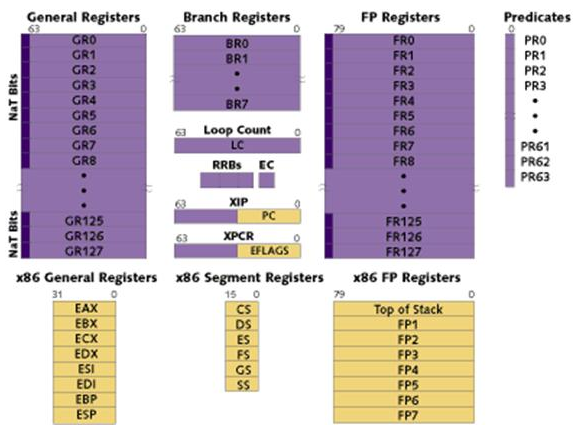
\includegraphics[scale=0.4]{2.png}
		\caption{Organización General} 
	\end{center}
\end{figure}
Los registros de gran longitud eliminan la complejidad del hardware, reducen la expansión del código fuente usando también los registros rotativos y mejora el desempeño reduciendo el acceso a la data de la cache.

Los registros son los siguientes:
\begin{enumerate}
\item 128 registros de enteros, cada uno de 64 bits de longitud.
\item 128 registros de punto flotante, cada uno de 80 bits de longitud.
\item 64 bits para la predicación.
\item 256 NAT bits.
\item 8 registros de ramificación.
\item 3 RRB's o registros base rotativos.
\item el LC.
\item y el EC.
\end{enumerate}
Todos los registros pueden ser accedidos por software, ya que son visibles al programador y de acceso aleatorio.

\subsubsection{Instrucciones}
El nuevo ISA de 64-bits usa la especulación, un método que permite al procesador iniciar la carga anticipadamente, incluso antes de que se sepa que va a ser utilizada.

Y que si el recibidor del banco pudiera identificar a los nuevos clientes del banco? Si el recibidor proveera los documentos para abrir una nueva cuenta por adelantado a todos los clientes que entren al banco, los clientes tendrían la oportunidad de terminar de rellenar los documentos para el momento que lleguen a la ventanilla. Si ellos no necesitan la solicitud, entonces ellos pueden devolver el documento mientras que legan a la cabecera de la cola, devolviéndola sin uso. Esto es comparable a como funciona la especulación. Las cargas de memoria son inicializadas por adelantado para asegurar que la data esta disponible para su uso. Como resultado, el compilador planifica la carga de memoria sin aguantar al procesador o bajar el rendimiento de éste.


Formato de las instrucciones del IA-64:
\begin{enumerate}
	\item Código de operación.
	\item Registro de predicado (6 bits)
	\item Registro fuente 1 (7 bits)
	\item Registro fuente 2 (7 bits)
	\item Registro destino (7 bits)
	\item Campos especiales para la aritmética entera y de punto flotante.
	\item Miscelánea.
\end{enumerate}

\subsection{Técnicas y Conceptos innovadores}
Las técnicas innovadoras de mejoramiento de desempeño como paralelismo explícito, predicación y especulación están explicadas a continuación:
\subsubsection{Paralelismo Explícito}
Para ilustrar las limitaciones de la arquitectura y de los beneficios del nuevo ISA de 64-bits, piensen como si un procesador estuviera operando como una sala de espera. Imaginen que nuestro banco tiene un recibidor el cual dirige a la gente a las diferentes líneas de servicio que se ofrece en nuestro banco, pudiendo ser a la línea de préstamo, retiros, etc. Esto es similar a lo que el compilador hace con el código, él lo organiza para su procesamiento. Sin embargo, en arquitecturas tradicionales, el recibidor es lento y solo puede organizar poca gente a la vez. Aún más, imaginen que el recibidor no esta seguro de que líneas hacen que cosa. Como resultado, los empleados en de las ventanillas tienen que redireccionar a los clientes. Esto requieres de trabajo a parte de que no es nada eficiente. Esto es una analogía de cómo es que operan las arquitecturas tradicionales.

\

En el paralelismo explícito, nuestro recibidor del banco realmente entiende las operaciones. Así que direcciona a los clientes a las ventanillas correctas y es tan eficiente que él puede llamar a las casas de los clientes para programar la entrevista por adelantado.

\

Esto hará que los clientes sepan exactamente a donde deben de ir, quitándole carga a nuestro recibidor. Ahora, el recibidor tiene mas libertad para programar a los clientes, maximizando el numero que puede ser atendidos. Este es el concepto detrás de paralelismo explícito, el compilador organiza eficientemente el código y hace explícito el pedido para que de esta manera el procesador pueda enfocarse en la ejecución de las instrucciones de manera mas efectiva.

\

\subsubsection{Predicación}
Normalmente, un compilador cambia una expresión de ramificación del código fuente (como lo es el IF-THEN-ELSE) en bloques alternados de código de maquina arreglados como un flujo secuencial. Dependiendo del resultado de la ramificación, el CPU ejecutara uno de los bloques básico salteándose los otros.

\

Predicación es un método de manejar ramificaciones condicionales. La idea principal del método es que el compilador planifique ambos caminos posibles de la ramificación para que sea ejecutada en el procesador simultáneamente.

\subsubsection{Especulación}
El retrieve de memoria, el tiempo de retorno de la data desde la memoria, es otra de las limitaciones de las arquitecturas tradicionales. Si el tiempo de traer la data desde la memoria fuese una operación bancaria, seria análoga a abrir una cuenta, la cual toma un poco de tiempo. Cuando un nuevo cliente abre una cuenta, aguanta toda la cola mientras que llenan los documentos en la ventanilla. De igual forma, el retrieve de memoria aguanta al procesador, dejándolo inactivo hasta que llegue la data desde la memoria. Debido al retrieve de memoria, no se esta conservando la velocidad del procesador, las cargas (la obtención de los datos desde la memoria) necesitan ser inicializados mas temprano para asegurar que la data llegue a tiempo para su uso.

\subsection{¿Qué aplicaciones se benefician de las arquitecturas de 64 bits?}
\begin{enumerate}
	\item Grandes bases de datos
	\item Software de modelado y simulación científica y de negocios
	\item Software intensivo de gráficos (CAD, juegos 3D)
	\item Criptografía
\end{enumerate}

\subsection{Desventajas de EPIC}
\begin{enumerate}
	\item Escribir los compiladores que sean capaces de estas sofisticadas optimizaciones ha resultado bastante más complejo de lo esperado.
	\item El Itanium 2 tiene una cifra exorbitante de 221 millones de transistores que disipan 130W de potencia. Como base de comparación, un Athlon
	XP tiene 54M transistores, y un Athlon 64 tiene 106M.
\end{enumerate}
\section{Conclusión}
Durante esta investigación hemos concluido que las arquitecturas de VLIW y EPIC son excelentes arquitecturas que nos otorgan mayor velocidad de procesamiento al utilizar el paralelismo de una sin embargo uno de los proncipales defectos que posee la arquitectura primitiva es su gran dependencia con los compiladores. Ademas cabe resaltar que EPIC es la evolución de VLIW, si bien es cierto EPIC mejora el rendimiento que VLIW pero aun así esta ligado a la desventaja del compilador.

Aun así no deja de ser una buena arquitectura que debe ser tomada en cuenta durante la evolución de las arquitecturas de los procesadores.

\end{document}